\section{Resultados}
\label{sec:resultados}
\subsection{Validación de los modelos}
\label{subsec:validacionModelos}

Esta sección se centrará en validar los diferentes modelos obtenidos en las secciones anteriores, específicamente la calculadora desarrollada en el cálculo analítico (\ref{sec:analitico}) y el modelo de cálculo por elementos finitos (\ref{sec:simulaciones}).

Los resultados de ambos modelos se presentan en forma de gráficas que muestran la evolución de la fuerza de atracción magnética. En el caso del cálculo analítico, la fuerza se expresa en función de la posición del vástago, mientras que en el modelo de elementos finitos, se expresa en función del tiempo. Aunque estas parecen ser variables independientes diferentes, ambas gráficas pueden considerarse análogas, ya que la única variable que varía en el sistema físico es la posición del vástago, midiéndola directamente en el primer modelo y observando su evolución temporal en el otro.

Esto implica que la evolución de la fuerza en ambas gráficas debería ser muy similar. Aunque se ha mencionado anteriormente que la magnitud del cálculo mediante elementos finitos no es precisa, podemos comparar las gráficas de las figuras \ref{fig:calcFsetupBase} y \ref{fig:S3ForceCurrent} para comprobar que, efectivamente, la evolución del parámetro de fuerza de atracción sigue el mismo patrón.

\begin{figure}[htbp]
    \centering
    \begin{minipage}{0.85\textwidth}
        \centering
        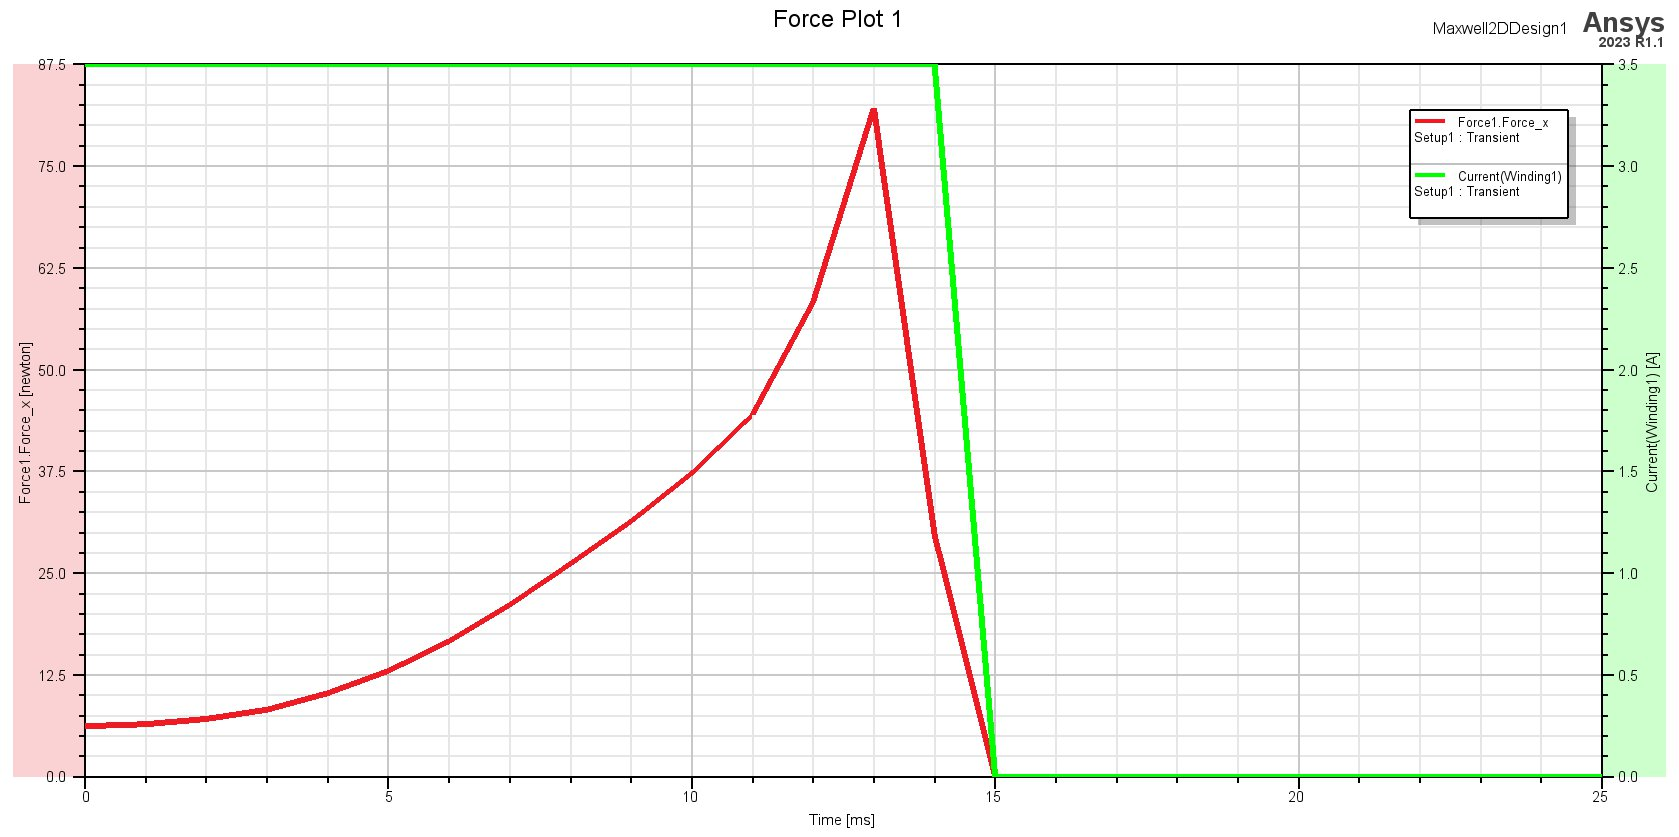
\includegraphics[width=\textwidth]{FigurasMemoria/S3ForceCurrent.jpg}
    \end{minipage}
    \hfill
    \begin{minipage}{0.9\textwidth}
        \centering
        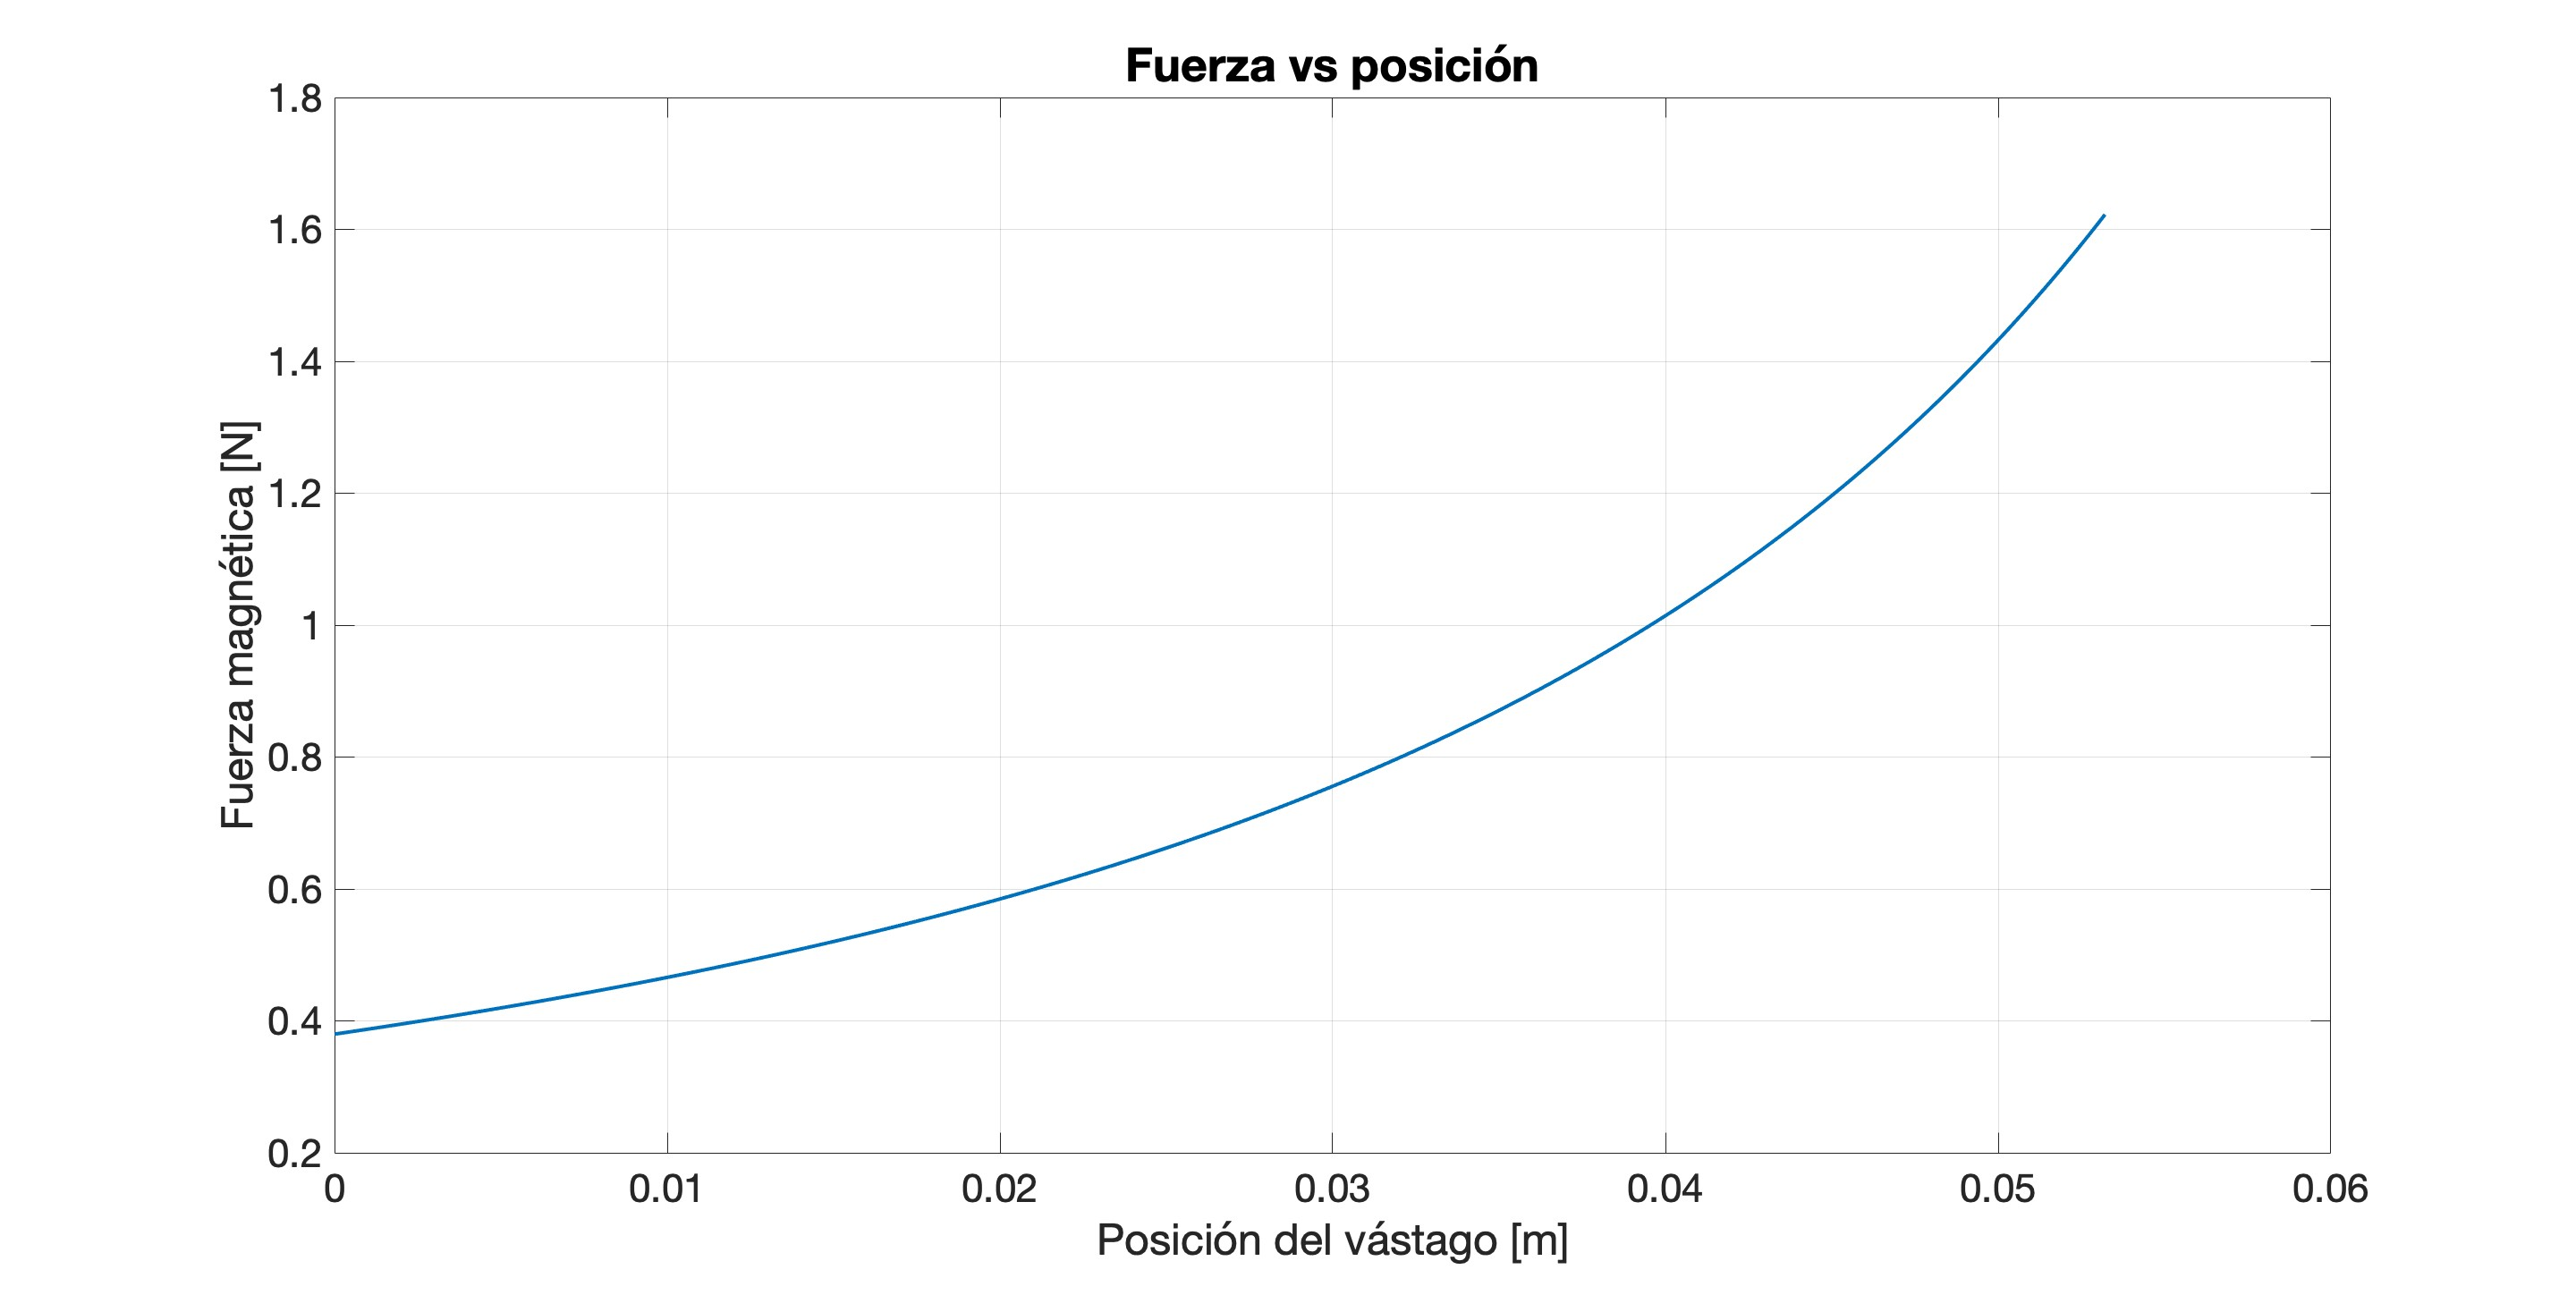
\includegraphics[width=\textwidth]{FigurasMemoria/calcFsetupBase.jpg}
    \end{minipage}
    \caption{Comparación de las figuras \ref{fig:calcFsetupBase} y \ref{fig:S3ForceCurrent}.}
    \label{fig:comparacionF}
\end{figure}

Como observamos en esta figura, la evolución de ambas gráficas muestra una curva ascendente, alcanzando el valor máximo de fuerza en el último momento de alimentación de la bobina. La gráfica de la figura \ref{fig:calcFsetupBase} no decrece porque no está computado lo que ocurre después de que \textit{x} llegue a su valor máximo. Sin embargo, este máximo del parámetro de posición del vástago coincide con el cese de la alimentación de la bobina, por lo que la fuerza se haría cero instantes después.

Como última observación, se puede notar en la gráfica del cálculo por elementos finitos que, al estar en un orden de magnitud de tiempo tan pequeño, ocurre un estado transitorio desde que la fuente deja de proporcionar corriente a la bobina hasta que esta realmente deja de emitir campo magnético. Esto se debe a la expresión de la evolución de la tensión y corriente en un solenoide:

\[V_L=L\frac{\partial i}{\partial t}\]

Lo que indica que existe una resistencia a la desaparición de la corriente en estos dispositivos debido a su tendencia de retener campo magnético.

Dado que el modelo analítico proporciona una aproximación mucho más certera tanto del valor de la fuerza como de su evolución, se concluye que ha sido exitoso su desarrollo y será el que se presente a los alumnos como método de comprobación de su elección de parámetros en el apartado de la práctica (\ref{sec:practica}).

\subsection{Resultados del prototipo}
\label{subsec:prototipoResults}

Los resultados del prototipo consisten en una serie de mediciones con diferentes geometrías de bobinas y valores de alimentación de las mismas. Se detallarán a continuación las diferentes configuraciones probadas y se discutirá si se puede explicar efectivamente las variaciones con el modelo propuesto en el apartado anterior. Las geometrías de las bobinas que se van a probar son:

\begin{table}[H]
    \centering
    \setlength{\tabcolsep}{5pt}
    \renewcommand{\arraystretch}{1.2}
    \begin{tabular}{|c|c|c|c|c|c|c|c|}
        \hline
        \textbf{Configuración} & \textbf{N} & \textbf{\(h_c\) [mm]} & \textbf{\(r_{cext}\) [mm]} & \textbf{\(r_{cint}\) [mm]} & \textbf{\(r_{cu}\) [mm]} & \textbf{\(l_{fe}\) [mm]} & \textbf{\(r_{fe}\) [mm]} \\
        \hline
        Base & 500 & 53,21 & 16,40 & 6,04 & 0,80 & 96,00 & 3,05 \\
        1 & 750 & 87,20 & 13,00 & 5,75 & \textbf{1,3} & 131,00 & 5,00 \\
        2 & 500 & 78,31 & 18,91 & 12,53 & 1,00 & 10,00 & 8,50 \\
        3 & 300 & 81,66 & 14,21 & 8,00 & 1,3 & 10,00 & 5,00 \\
        \hline
    \end{tabular}
    \caption{Configuraciones de bobinas a probar.}
    \label{tab:geometrias}
\end{table}

\newpage

\newgeometry{left=1.5cm, right=1.5cm, top = 2.5cm, bottom = 2.5cm}

\begin{table}[H]
    \centering
    \setlength{\tabcolsep}{5pt}
    \renewcommand{\arraystretch}{1.2}
    \begin{tabular}{|c|c|c|c|}
        \hline
        \textbf{Alimentación} & \textbf{Tensión [V]} & \textbf{Resistencia [\(\Omega\)]} & \textbf{Corriente [A]}\\
        \hline
        1 & 13,1 & 3,5 & 3,74 \\
        2 & 20,0 & 3,5 & 5,71 \\
        3 & 29,7 & 3,5 & 8,49\\
        \hline
    \end{tabular}
    \caption{Denominación de las diferentes alimentaciones.}
    \label{tab:alimentacionesBase}
\end{table}

\begin{table}[H]
    \centering
    \begin{tabular}{|c|c|c|c|c|}
    \hline
    \setlength{\tabcolsep}{5pt}
    \renewcommand{\arraystretch}{1.2}
    \textbf{Alimentación} & \textbf{Tiempo [ms]} & \textbf{Distancia [m]} & \textbf{Velocidad [ms\(^{-1}\)]} & \textbf{Aceleración [ms\(^{-2}\)]} \\
    \hline
    \renewcommand{\tabcolsep}{6pt}
    \renewcommand{\arraystretch}{1.0}
    \multirow{10}{*}{1} & 27     & \multirow{10}{*}{0,0691} & 2,16      & 67,48       \\
                        & 22     &                          & 2,09      & 63,45       \\
                        & 24     &                          & 2,09      & 63,45       \\
                        & 38     &                          & 2,09      & 63,45       \\
                        & 25     &                          & 2,09      & 63,45       \\
                        & 33     &                          & 2,03      & 59,78       \\
                        & 24     &                          & 1,97      & 56,41       \\
                        & 28     &                          & 2,23      & 71,9        \\
                        & 25     &                          & 2,09      & 63,45       \\
                        & 31     &                          & 2,09      & 63,45       \\
    \hdashline[2pt/5pt]
    \multirow{10}{*}{2} & 18     & \multirow{10}{*}{0,0691} & 2,47      & 88,14       \\
                        & 18     &                          & 2,66      & 102,22      \\
                        & 18     &                          & 2,47      & 88,14       \\
                        & 21     &                          & 2,47      & 88,14       \\
                        & 19     &                          & 2,56      & 94,79       \\
                        & 25     &                          & 2,56      & 94,79       \\
                        & 18     &                          & 2,56      & 94,79       \\
                        & 25     &                          & 2,56      & 94,79       \\
                        & 17     &                          & 2,66      & 102,22      \\
                        & 22     &                          & 2,56      & 94,79       \\
    \hdashline[2pt/5pt]
    \multirow{10}{*}{3} & 21     & \multirow{10}{*}{0,0691} & 2,47      & 88,14       \\
                        & 20     &                          & 2,56      & 94,79       \\
                        & 20     &                          & 2,56      & 94,79       \\
                        & 19     &                          & 2,66      & 102,22      \\
                        & 21     &                          & 2,56      & 94,79       \\
                        & 23     &                          & 2,56      & 94,79       \\
                        & 22     &                          & 2,47      & 88,14       \\
                        & 20     &                          & 2,56      & 94,79       \\
                        & 22     &                          & 2,56      & 94,79       \\
                        & 23     &                          & 2,47      & 88,14       \\
    \hline
    \end{tabular}
    \caption{Datos tomados con la bobina base y las alimentaciones de la tabla \ref{tab:alimentacionesBase}.}
    \label{tab:datosBase}
\end{table}

\begin{table}[H]
    \centering
    \setlength{\tabcolsep}{5pt}
    \renewcommand{\arraystretch}{1.2}
    \begin{tabular}{|c|c|c|c|}
        \hline
        \textbf{Alimentación} & \textbf{Vel. Media [ms\(^{-1}\)]} & \textbf{Ac. Media [ms\(^{-2}\)]} & \textbf{Fuerza [N]} \\
        \hline
        1 & 2,53 & 92,49 & 1,76 \\
        2 & 3,47 & 174,31 & 3,31 \\
        3 & 3,28 & 155,8 & 2,96 \\
        \hline
    \end{tabular}
    \caption{Resultados del disparo con la bobina base y las alimentaciones de la tabla \ref{tab:alimentacionesBase}.}
    \label{tab:resultadosBase}
\end{table}
\restoregeometry

Con estos resultados, podemos terminar de validar la simulación ejecutada para obtener las figuras \ref{fig:calcRsetupBase}, \ref{fig:calcBsetupBase} y \ref{fig:calcFsetupBase}.